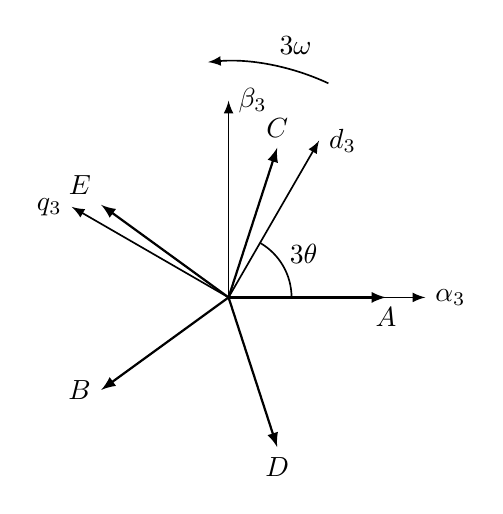
\begin{tikzpicture}[>=latex, line width=0.6pt]
\begin{scope}[shift={(7,0)}]
    % Osy alpha a beta
    \draw[->] (0,0) -- (2.5,0) node[right] {$\alpha_3$};
    \draw[->] (0,0) -- (0,2.5) node[right] {$\beta_3$};
    
    % Vektory fází A-E
    \draw[->, thick] (0,0) -- (0:2) node[below] {$A$};
    \draw[->, thick] (0,0) -- (216:2) node[left] {$B$};
    \draw[->, thick] (0,0) -- (72:2) node[above] {$C$};
    \draw[->, thick] (0,0) -- (288:2) node[below] {$D$};
    \draw[->, thick] (0,0) -- (144:2) node[above left] {$E$};
    
    % d-q soustava
    \def\threetheta{60}
    \draw[->] (0,0) -- (\threetheta:2.3) node[right] {$d_3$};
    \draw[->, shift={(0,0)}] (0,0) -- (\threetheta+90:2.3) node[left] {$q_3$};
    
    % Úhel 3*theta
    \draw (\threetheta:0.8) arc (\threetheta:0:0.8);
    \node at (30:1.1) {$3\theta$};
    
    % ŠIPKA 3*OMEGA - nyní na poloměru 3.0 (velmi daleko)
    \draw[->] (65:3.0) arc (65:95:3.0) node[midway, above right] {$3\omega$};
    
\end{scope}

\end{tikzpicture}